%\subsection{Scaling and speedup comparison}

\subsection{Speedup on various references}
%\paragraph{Different reference graphs}
\cref{TRIEtab:results} shows the performance of optimal aligners across various
references. On all references, \astarix is consistently faster than \dijkstra,
which is consistently faster than \pasgal and \bitparallel. The memory usage of
\dijkstra is within a factor of 3 compared to \pasgal and \bitparallel. Due to
the heuristic memoization, the memory usage of \astarix can grow several times
compared to \dijkstra.

\begin{table}[H]
\centering
\ra{0.8}
\caption[Performance of optimal aligners for difference references]{Performance
of optimal aligners for different reference graphs.}\label{TRIEtab:results}
\sffamily
%\rowcolors{2}{gray!25}{white}

\renewrobustcmd{\bfseries}{\fontseries{b}\selectfont}
\renewrobustcmd{\boldmath}{}

\begin{tabular}{llrrrr}
\toprule
                && \multicolumn{4}{ c }{\textbf{Runtime} and \textbf{Memory}}\\
                \cmidrule{3-6}
\textbf{Genome graph} & \textbf{Size} & \bfseries \astarix & \dijkstra & \pasgal & \bitparallel\\
\midrule
    \rowcolor{gray!10}
    & &\bfseries \numprint{33} sec	 &\numprint{73} sec &\numprint{3272} sec &\numprint{4906} sec \\
    \rowcolor{gray!10}
    \multirow{-2}{*}{\textit{E. coli} (linear)} & \multirow{-2}{*}{4.7 Mbp} &\numprint{0.66} GB   &\numprint{0.66} GB &\numprint{0.55} GB   &\numprint{0.43} GB \\
    & &\bfseries \numprint{437} sec &\numprint{940} sec	 &\numprint{1614} sec & \\
    \multirow{-2}{*}{LCR (graph)} & \multirow{-2}{*}{1 Mbp} &\numprint{1.12} GB   &\numprint{1.09} GB &\numprint{0.30} GB   & \multirow{-2}{*}{SegFault}\\
    \rowcolor{gray!10}
    & &\bfseries \numprint{1282} sec &\numprint{1588} sec & >\numprint{7200} sec &\\
    \rowcolor{gray!10}
    \multirow{-2}{*}{MHC1 (graph)} & \multirow{-2}{*}{5 Mbp} &\numprint{4.35} GB   &\numprint{1.21} GB    &  \numprint{0.87} GB         		&\multirow{-2}{*}{SegFault}\\
\bottomrule
\end{tabular}

\end{table}

\subsection{Scaling with reference size}

\cref{TRIEfig:scaling_with_graphsize} compares the performance of existing optimal
aligners. \bitparallel and \pasgal always explore all states, thus their
average-case reaches the worst-case complexity of $\Oh(\lvert \AG \rvert) =
\Oh(m \concat \RG)$. Due to the trie indexing, the runtime of \astarix and
\dijkstra scales in the reference size with a polynomial of power around $0.2$
versus the expected linear dependency of \bitparallel and \pasgal.

The heuristic function of \astarix demonstrates a 2-fold speed-up over
\dijkstra. This is possible due to the highly branching trie structure, which
allows skipping the explicit exploration for the majority of starting nodes. 

\begin{figure}[t]
  \begin{subfigure}{.45\textwidth}
    \centering
    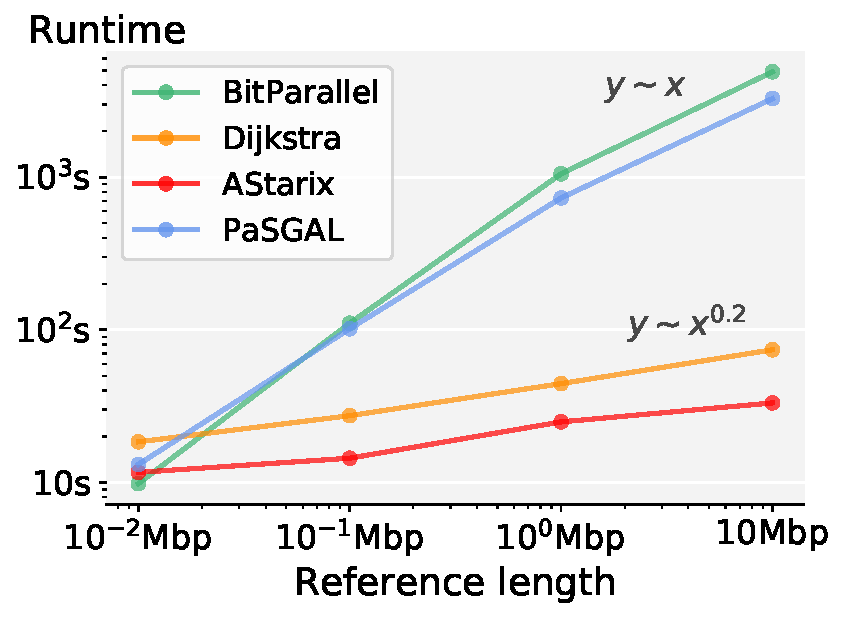
\includegraphics[width=\linewidth]{figs/cmp/performance_vs_genomesize-head_Mbpxs.pdf}
  \end{subfigure}
  \begin{subfigure}{.45\textwidth}
    \centering
    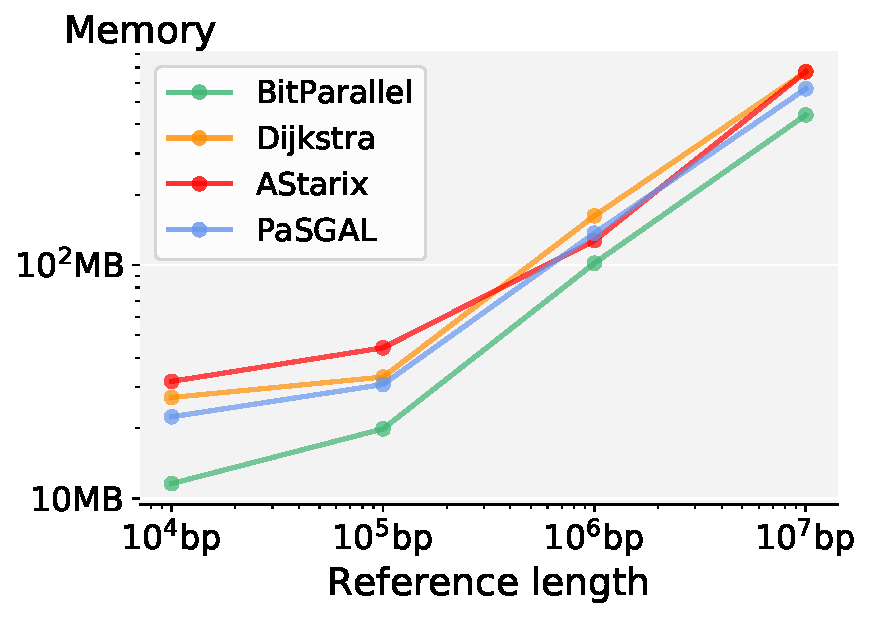
\includegraphics[width=\linewidth]{figs/cmp/memory_vs_genomesize-headxmax_rss.pdf}
  \end{subfigure}
  \caption[Performance scaling with reference size]{Comparison of overall
     runtime and memory usage of optimal aligners with increasing prefixes of E.
     coli as references}
  \label{TRIEfig:scaling_with_graphsize}
\end{figure}

\subsection{Scaling with number of errors}
To measure the speedup caused by the heuristic function, we compare the number
of not only the expanded, but also of explored states (the latter number is
never smaller, and the example in~\cref{TRIEfig:heuristic-benefit}) between
\astarix and \dijkstra on the MHC1 dataset.

\cref{TRIEfig:scaling_with_errors} demonstrates the benefit of the heuristic
function in terms of both alignment time and number of explored states. Most
importantly, \astarix scales much better with increasing number of errors in the
read, compared to \dijkstra. More specifically, the number of states explored by
\dijkstra, as a function of alignment cost, grows exponentially with a base of 
around 10, whereas the base for \astarix is around 3 (the empirical complexity is
estimated as a best exponential fit \mbox{$\mli{exploredStates} \sim a \cdot
\mli{score}^b$}).

The horizontal black line in \cref{TRIEfig:scaling_with_errors} denotes the total
number of states $\lvert \RG \rvert \cdot \lvert q \rvert$, which is always
explored by \bitparallel and \pasgal. On the other hand, any aligner must
explore at least $m = \lvert q \rvert$ states, which we show as a horizontal
dashed line. This lower bound is determined by the fact that at least the states
on a best alignment need to be explored.

\begin{figure}[t]
  \begin{subfigure}{.45\textwidth}
    \centering
    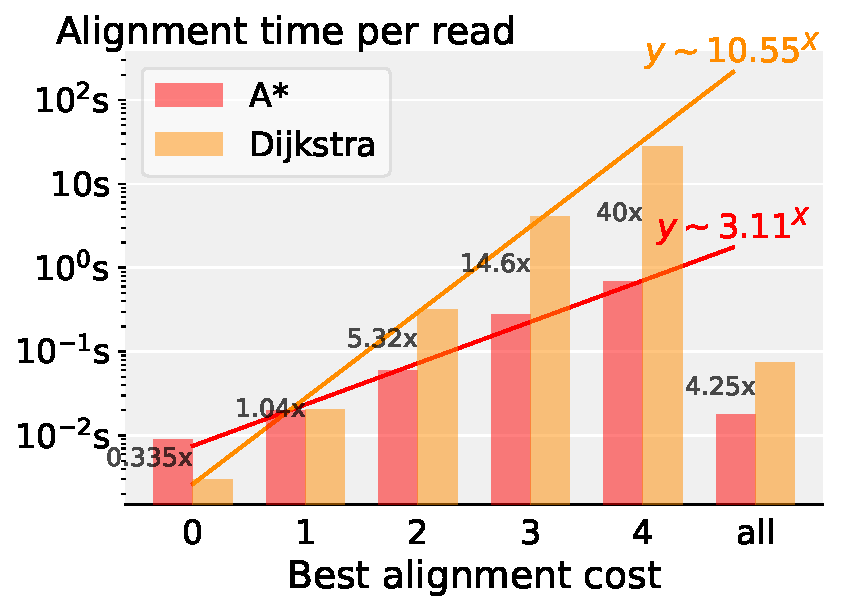
\includegraphics[width=\linewidth]{figs/cmp/heuristic_MHC1_cost-t(map).pdf}
  \end{subfigure}%~\hspace{1em}
  \begin{subfigure}{.45\textwidth}
    \centering
    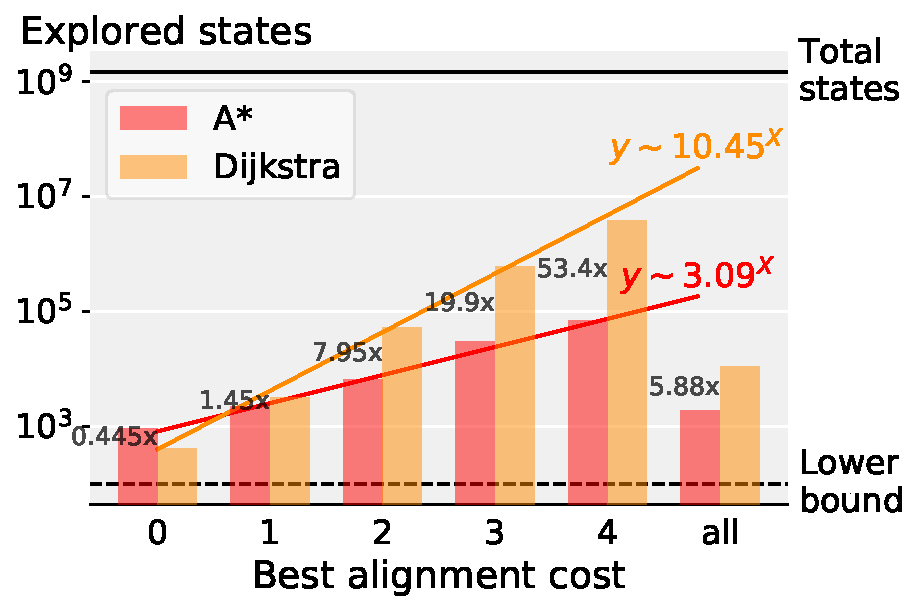
\includegraphics[width=\linewidth]{figs/cmp/heuristic_MHC1_cost-explored_states.pdf}
  \end{subfigure}%
  \caption[Performance scaling with alignment cost]{Comparison of \A and \dijkstra in terms of mean alignment runtime per read and mean explored states depending on the alignment cost on MHC1.}
  \label{TRIEfig:scaling_with_errors}
\end{figure}